\documentclass[twocolumn]{aastex61}

\newcommand{\vdag}{(v)^\dagger}
\newcommand\aastex{AAS\TeX}
\newcommand\latex{La\TeX}

%% Reintroduced the \received and \accepted commands from AASTeX v5.2
%\received{July 1, 2016}
%\revised{September 27, 2016}
%\accepted{\today}
\submitjournal{ApJL}

\shorttitle{Atmosphere Characterization of WASP-107\lowercase{b}}
\shortauthors{Kreidberg et al.}

\begin{document}

\title{Water, High-Altitude Condensates, and Methane Depletion in the Atmosphere of the Warm Neptune WASP-107\lowercase{b}}

\correspondingauthor{Laura Kreidberg}
\email{laura.kreidberg@cfa.harvard.edu}

\author{Laura Kreidberg}
\affiliation{Harvard Society of Fellows\
78 Mt. Auburn St.\\
Cambridge, MA 02138, USA}
\affiliation{Harvard-Smithsonian Center for Astrophysics\
60 Garden St.\\
Cambridge, MA 02138}
\nocollaboration

\author{Michael R. Line}
\affiliation{Arizona State University}
\nocollaboration

\author{Daniel Thorngren}
\affiliation{University of California Santa Cruz}
\nocollaboration

\author{Caroline V. Morley}
\altaffiliation{Sagan Fellow}
%\affiliation{Harvard-Smithsonian Center for Astrophysics}
\affiliation{Harvard-Smithsonian Center for Astrophysics\
60 Garden St.\\
Cambridge, MA 02138}
\nocollaboration

\author{Kevin B. Stevenson}
\affiliation{Space Telescope Science Institute}
\nocollaboration


\begin{abstract}
The Neptune-mass exoplanet WASP-107b is an exciting target for atmosphere characterization. It has an unusually large atmospheric scale height and a small, bright host star, raising the possibility of precise constraints on its current nature and formation history.  We report the first atmospheric study of WASP-107b, a Hubble Space Telescope measurement of its near-infrared transmission spectrum.  We determined the planet's composition with two techniques: atmospheric retrieval based on the transmission spectrum and interior structure modeling based on the observed mass and radius. We detect water at $6.5\,\sigma$ confidence and set an upper limit on the atmospheric metallicity of $30\times$ solar. We find that the methane abundance is depleted relative to expectations for a solar abundance pattern (at $3\,\sigma$ confidence), suggesting a low carbon-to-oxygen ratio or high internal heat flux.  The water features are smaller than expected for a cloudless atmosphere, crossing less than one scale height, and require a thick condensate layer at high altitudes (0.1 - 3 mbar). We find that it is challenging for physically motivated cloud and haze models to produce opaque condensates at these pressures.  Taken together, these findings serve as an illustration of the diversity and complexity of exoplanet atmospheres. The community can look forward to more such results with the high precision and wide spectral coverage afforded by future observing facilities. 
\end{abstract}

%% Keywords should appear after the \end{abstract} command. 
%% See the online documentation for the full list of available subject
%% keywords and the rules for their use.
\keywords{planets and satellites: individual (WASP-107b), planets and satellites: atmospheres}

%% From the front matter, we move on to the body of the paper.
%% Sections are demarcated by \section and \subsection, respectively.
%% Observe the use of the LaTeX \label
%% command after the \subsection to give a symbolic KEY to the
%% subsection for cross-referencing in a \ref command.
%% You can use LaTeX's \ref and \label commands to keep track of
%% cross-references to sections, equations, tables, and figures.
%% That way, if you change the order of any elements, LaTeX will
%% automatically renumber them.

%% We recommend that authors also use the natbib \citep
%% and \citet commands to identify citations.  The citations are
%% tied to the reference list via symbolic KEYs. The KEY corresponds
%% to the KEY in the \bibitem in the reference list below. 


\section{Introduction} \label{sec:intro}
The composition of a planet's atmosphere depends on where and how the planet formed. By measuring the inventory of atmospheric elemental abundances, we can shed light on important aspects of the formation process such as location within the disk and the relative accretion rates of gas versus solids \citep[][]{oberg11, fortney13, madhusudhan14, alidib16, mordasini16, espinoza17}.  

The warm Neptune WASP-107b is an intriguing target for atmosphere characterization for several reasons.  It has an intermediate size between ice giants and gas giants, with a mass similar to Neptune's and a radius close to Jupiter's \citep[$0.12\,M_\mathrm{Jup}$, $0.94\,R_\mathrm{Jup}$;][]{anderson17}. Studying the atmospheres of planets in this transition region will provide additional clues in the much-debated mystery of what stunts the growth of Neptune-size planets \citep[e.g][]{pollack96, dawson16, frelikh17}.  

WASP-107b also has a relatively low equilibrium temperature compared to most other exoplanets that are amenable to atmosphere characterization (780 K, assuming zero albedo).  This results in a distinct atmospheric chemistry from other well-studied systems: at low temperatures, the dominant molecular reservoir for carbon transitions from carbon monoxide to methane \citep{moses13}.  Spectral features from both water and methane are accessible with current observing facilities, enabling a spectroscopic estimate of the carbon-to-oxygen ratio (C/O). Previous measurements of C/O have been challenging because they rely on broadband photometry or narrow wavelength coverage \citep[e.g.][]{madhusudhan11, line14, benneke15, kreidberg15b}. 

In addition, WASP-107b is one of the best targets discovered to date for atmosphere characterization. Thanks to its large atmospheric scale height and small, bright host star, the expected signal-to-noise for the transmission spectrum is comparable to the best studied benchmarks in the field (e.g. HD\,209458b).  In this paper we report the first atmosphere characterization of WASP-107b: a near-infrared transmission spectrum measured with the \emph{Hubble Space Telescope} (\emph{HST}; Program GO 14915, PI L. Kreidberg).

\section{Observations and Data Reduction}
We observed a single transit of WASP-107b with \emph{HST}'s Wide Field Camera 3 (WFC3) instrument on UT 5-6 June 2017.  The transit observation consisted of five \emph{HST} orbits. At the beginning of each 96-minute orbit, we took an image of the target with the F130N filter (exposure time = 4.2 s). This direct image is used for wavelength calibration. For the remainder of the target visibility period (about 45 minutes), we obtained time series spectra with the G141 grism, which provides low-resolution spectroscopy over the wavelength range $1.1 - 1.7\,\mu$m.  We used the NSAMP=6, SPARS\_25 readout mode (exposure time = 112 s) to optimize the efficiency of the observations, as determined by the \texttt{PandExo\_HST} planning tool\footnote{\url{https://github.com/spacetelescope/PandExo\_HST}}.  As is standard for WFC3 observations of bright targets, we used the spatial scanning observing mode, which slews the telescope in the spatial direction over the course of an exposure. The scan rate was 0.12 arcseconds/sec.

We reduced the data with the custom pipeline described in \cite{kreidberg14a}, which we summarize briefly here. For each exposure, we extracted the spectrum from each up-the-ramp sample (or ``stripe") separately using the optimal extraction algorithm of \cite{horne86}. The stripe spectra were then summed to create the final spectrum. For each stripe, the extraction box was 80 pixels high and centered on the stripe's midpoint in the spatial direction. We corrected the spectra for the changing dispersion solution over the length of the spatial scan and small drifts over time ($<0.1$ pixel).  To subtract the background, we took the median of sky pixels that were uncontaminated by the target spectrum (rows $5-250$, columns $5-15$). 
%dispersion solution: 46 Angstroms/pixel. max drift: 3 angstroms (from diagnostics.txt)

\section{Light Curve Analysis}
The data analysis had two parts: the band-integrated ``white" light curve fit and the spectroscopic light curve fits.

\subsection{White Light Curve}
To create the raw white light curve, we summed each spectrum over the 181 pixels in the spectral trace.  The white light curve has systematic trends that are typical for WFC3 observations \citep{zhou17}: the flux increases asymptotically over each orbit (the ``ramp" effect) and there is a visit-long linear trend. The largest ramp occurs in the initial orbit (orbit zero), so we only fit data from orbits one through four in our analysis, following common practice.  We fit the light curve with the analytic model of the form $F_\mathrm{white}(t) = S_\mathrm{white}(t)\times T_\mathrm{white}(t)$, where $S_\mathrm{white}$ is a systematics model and $T_\mathrm{white}$ is a transit model. We used the same systematics model as \cite{kreidberg15b}.  We modelled the transit with the \texttt{batman} package \citep{kreidberg15a}.  The model parameters are the orbital period $p$, time of inferior conjunction $t_0$, transit depth $r_p/r_s$, ratio of semi-major axis to stellar radius $a/r_s$, orbital inclination $i$, and the quadratic stellar limb darkening parameters $u_1$ and $u_2$.

\begin{figure*}
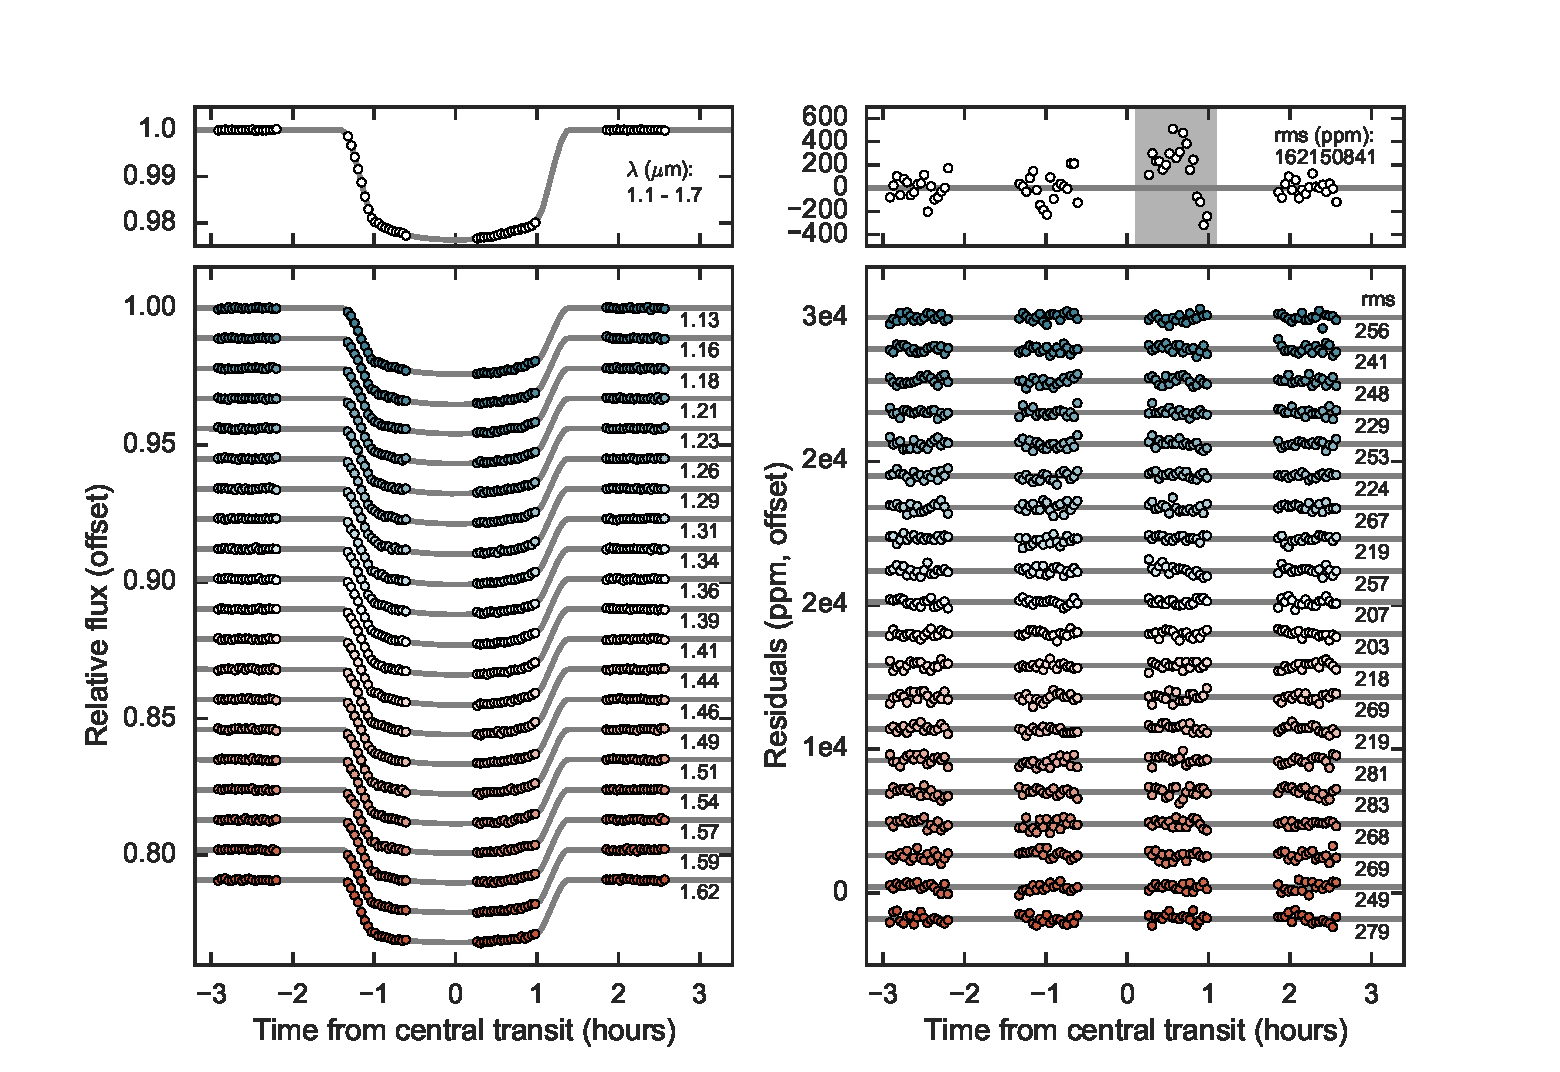
\includegraphics[width = \textwidth]{Figures/lc.pdf}
\caption{Left: Broadband and spectrophotometric transit light curves for WASP-107b compared to best fit models. Right: residuals from the best fit. Annotations indicate the central wavelength and root-mean-square (rms) residuals. A star-spot crossing feature is shaded in gray in the upper right; our systematic error correction removes this feature from the spectroscopic light curves.} 
\label{fig:lc}
\end{figure*}

\subsubsection{Star Spot Crossing}
In our initial analysis, we noticed a bump in the light curve during orbit three that was not fit well with our model. We attribute this feature to a star spot crossing event, as WASP-107 is an active star and spot crossings have been observed before \citep{dai17, mocnik17}. In our subsequent analysis, we gave the data in orbit three no weight in the fit. The amplitude of the spot crossing feature is 300 ppm, as illustrated in Figure\,\ref{fig:lc}.

\subsubsection{Final Fit}
In our final fit, we fixed the transit parameters $a/r_s$, $i$, $p$ on the precise estimates from the Kepler light curve \citep{dai17}.  We also fixed the limb darkening parameters on predictions from a PHOENIX model for a star with effective temperature 4300 K, calculated with the \texttt{limb-darkening} package from \cite{espinoza15}.  We checked that the values we fixed were consistent with our estimates when we allowed them to vary freely.  We also checked that the uncertainty in the stellar parameters does not significantly affect the PHOENIX model predictions at the level of precision of our data.  The remaining free parameters in the fit were $t_0$, $r_p/r_s$, and the systematics parameters for the visit-long and orbit-long trends.

For the best fit white light curve, the root-mean-square (rms) residuals were 93 ppm (excluding the star spot crossing), which is somewhat larger than the expected shot noise of 50 ppm. We attribute the excess noise to loss of flux off the edge of the detector, which can occur if there is variation in the position or length of the spatial scan. There is no evidence for correlated noise in the residuals, so to account for the excess noise we simply increased the per-point uncertainties by a factor of 1.7 to achieve a $\chi^2_\nu$ value of unity.  We then used the Markov chain Monte Carlo (MCMC) algorithm to estimate parameter uncertainties \citep{foremanmackey13}.  The chain had 50 walkers which each ran for $10^4$ steps with the first 10\% discarded as burn-in. We tested for convergence by dividing the chain in two halves and confirming that they gave consistent results. The transit time was $t_0 = 2457910.45407\pm6\mathrm{e}{-5}$ BJD$_\mathrm{TDB}$ and the planet/star radius was $r_p/r_s = 0.14399\pm0.00017$. 

\subsection{Spectroscopic Light Curve Fits}
We binned the spectrum into 20 spectrophotometric channels from 1.12 to 1.65 $\mu$m, shown in Figure\,\ref{fig:lc}. We fit the light curves with the \texttt{divide-white} technique, which assumes that the light curve systematics have the same morphology at all wavelengths \citep{stevenson14c, kreidberg14a}. For this method, the transit model $T_\lambda(t)$ is multiplied by the systematics vector from the white light curve fit ($F_\mathrm{white}/T_\mathrm{white}$), and rescaled by a factor $C_\lambda + V_\lambda t$.  One advantage of this approach is that it removes the star spot crossing feature, enabling us to use orbit three with no additional correction. The amplitude of the feature has no detectable wavelength dependence at the level of precision of our data.  As for the white light curve, we fixed some of the transit parameters on the estimates from \cite{dai17} and fixed the limb darkening on the PHOENIX model. The final spectroscopic light curve fits had just three free parameters: $C_\lambda$, $V_\lambda$, and $r_p/r_s$.  

The best fit light curves have a median $\chi^2_\nu$ value of 1.16.  We conservatively rescaled the photometric uncertainties for all spectroscopic channels such that the $\chi^2_\nu$ values are unity. We performed an MCMC fit to the light curves with \texttt{emcee}.  For each light curve we ran a fit with 50 walkers and 1000 steps per walker, and tested for convergence as we did for the white light curve. The median transit depths and $1\,\sigma$ uncertainties are given in Table\,\ref{tab:transit_depths}. 

We explored several alternative choices for the spectroscopic light curve fits, but found that none of them made a significant difference in the transmission spectrum. For example, we fit the spectroscopic light curves with the same analytic model we used for the white light curve and obtained nearly identical relative transit depths. 
%(differing by just $0.3\sigma$ on average), except with a small constant offset due to the uncorrected star-spot crossing feature. This offset does not affect our final analysis because it is marginalized in the atmospheric retrieval (see \S\,\ref{sec:retrieval}). 
We also fit for a linear limb darkening parameter rather than fixing the limb darkening on the PHOENIX model values. We found that the fitted limb darkening coefficients are consistent with the model predictions, so we opted to fix the coefficients in our final analysis because it improves the precision on the transit depths by about 10\%.  We also performed an independent data reduction and fit using K. Stevenson's pipeline and found consistent results (well within $1\,\sigma$). 

%\subsubsection{Transit Depths Redder than 1.62 $\mu$m}
%The red edge of the transmission spectrum is of interest for our analysis because methane is expected to be the dominant absorber over water at wavelengths greater than $1.6\,\mu$m. Unfortunately, we find that the our reddest spectroscopic light curves ($>1.62\mu$m) are too poor in quality to robustly measure the transit depth. The residuals exhibit correlated noise and the fits have $\chi^2_\nu>2$. The transit depths are also sensitive to which method we use to fit for instrument systematics.  We therefore opt not to report transit depths redder than the 1.62 $\mu$m channel.


\begin{figure*}
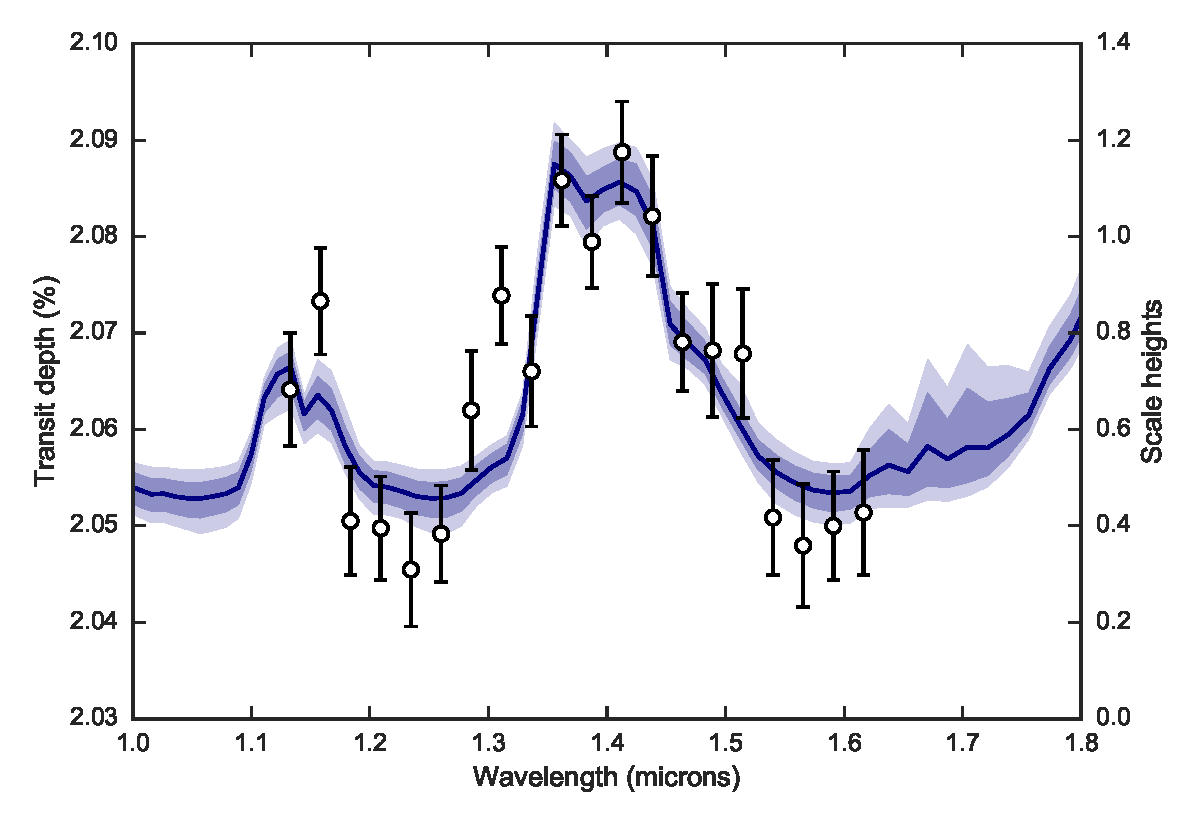
\includegraphics[width = \textwidth]{Figures/spectrum.pdf}
\caption{The transmission spectrum of WASP-107b (points with 1\,$\sigma$ error bars) compared to retrieved models (blue line with shaded $1$ and $2\sigma$ confidence intervals). The features at $1.15$ and $1.4$ $\mu$m are due to water absorption. The right-hand axis indicates the normalized atmospheric scale height assuming a $10\times$ solar composition. The water feature crosses less than one scale height, indicating that condensates are present at high altitude.} 
\label{fig:spectrum}
\end{figure*}

\begin{deluxetable}{c c c}
\tablecaption{WASP-107b transmission spectrum \label{tab:transit_depths}}
\tablehead{\colhead{Wavelength ($\mu$m)}  & \colhead{Transit depth} & \colhead{Uncertainty}}
\startdata
1.133 & 0.020641 & 5.9e-05 \\
1.158 & 0.020733 & 5.5e-05 \\
1.184 & 0.020505 & 5.6e-05 \\
1.209 & 0.020498 & 5.4e-05 \\
1.235 & 0.020455 & 5.9e-05 \\
1.260 & 0.020492 & 5.0e-05 \\
1.285 & 0.020620 & 6.2e-05 \\
1.311 & 0.020739 & 5.0e-05 \\
1.336 & 0.020660 & 5.7e-05 \\
1.362 & 0.020858 & 4.8e-05 \\
1.387 & 0.020794 & 4.8e-05 \\
1.413 & 0.020888 & 5.2e-05 \\
1.438 & 0.020821 & 6.2e-05 \\
1.464 & 0.020691 & 5.1e-05 \\
1.489 & 0.020682 & 6.9e-05 \\
1.515 & 0.020679 & 6.7e-05 \\
1.540 & 0.020509 & 6.0e-05 \\
1.565 & 0.020480 & 6.4e-05 \\
1.591 & 0.020500 & 5.6e-05 \\
1.616 & 0.020514 & 6.5e-05 \\
\enddata
\end{deluxetable}

\section{Composition of the Atmosphere}
In this section we discuss constraints on the composition of WASP-107b's atmosphere based on interior structure modeling and atmospheric retrieval of the measured transmission spectrum.

\subsection{Atmospheric Metallicity from Interior Structure Modeling}
\label{sec:interior}
Given WASP-107b's unusually low density, we quantitatively explored the range of atmospheric metallicities that are consistent with the observed mass and radius using the structure evolution modeling of \cite{thorngren16}.  These models assume a thermally inert heavy-element core with a convective envelope of additively mixed H/He \citep{saumon95} and heavy-element impurities.  The heavy elements were a 50-50 rock-ice mix. We evolved the planets in time using the atmospheric models of \cite{fortney07}.  The results are sensitive to assumptions about the stellar age, which is uncertain \citep[either $0.6\pm0.2$ to $8.3\pm4.3$ Gyr depending on model assumptions;][]{mocnik17}. We therefore ran two models, with uniform age priors of either $0.2-1.0$ or $1.0-13.8$ Gyr.  We used the published mass and radius estimates \citep[$0.12\pm0.01\,M_\mathrm{J}$, $0.94\pm0.02$;][]{anderson17}.  %A more precise mass estimate is in preparation (B. Benneke, priv.\,comm.); however, we find that our results are not significantly affected when we vary the assumed mass by $\pm3\,\sigma$ from the published value because the dominant uncertainties are the stellar age and core mass.

Based on these assumptions, we fit for envelope metallicity and core mass using an MCMC with uniform priors on both parameters.  The MCMC burned in for $10^3$ steps and then collected $4\times10^6$ samples.  The envelope metal mass fractions were converted to metallicities assuming the mean molecular weight of the metals was 18 (the value for water), using the approach of \cite{fortney13}. Figure\,\ref{fig:metal_prior} shows the results.  We find a $3\,\sigma$ upper limit on the metallicity of $30\times$ solar for the young stellar age range.  Higher metallicity envelopes are not allowed because they decrease the planet's radius below the observed value.  For the older age, the upper limit is even lower ($20\times$ solar), because planets cool and contract as they age \citep{fortney08}.  These are conservative upper limits, but realistically, the planet probably formed with a core. Assuming a $5\,M_\oplus$ core, the upper limit on metallicity is 20 (10) $M_\oplus$ for the young (old) age.  

\begin{figure}
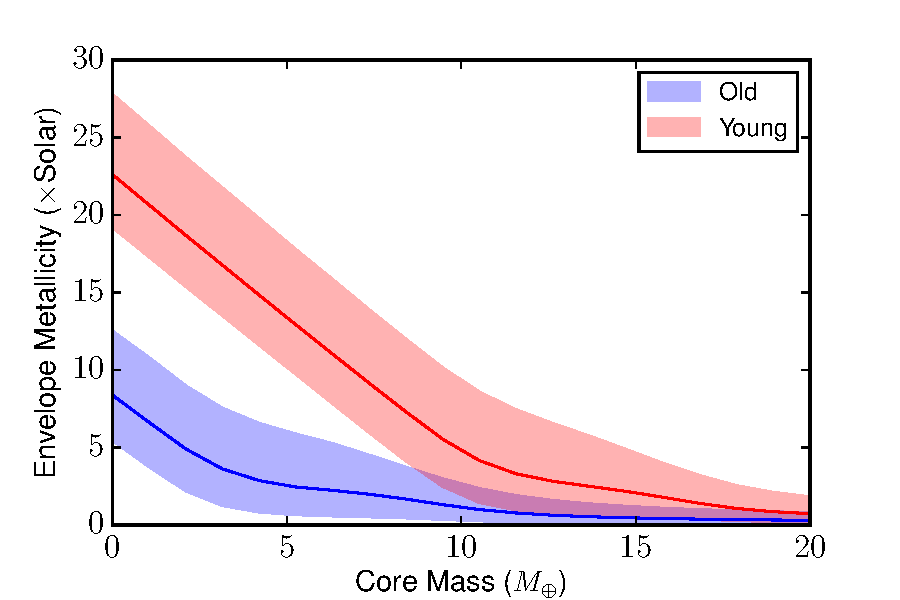
\includegraphics[width = 0.5\textwidth]{Figures/metalByAge.pdf}
\caption{Estimated envelope metallicity for a given core mass based on interior structure modeling. The red shading corresponds to the $1\sigma$ confidence interval for a young planet ($0.2-1$ Gyr); the blue is for an older age ($1-14$ Gyr).}
\label{fig:metal_prior}
\end{figure}

\subsection{Retrieval}
\label{sec:retrieval}
We also inferred the composition of the atmosphere directly from the transmission spectrum using the CHIMERA chemically-consistent retrieval \citep{line13a}.   Briefly, CHIMERA solves the transmission geometry problem using the equations in \cite{brown01, tinetti12}.  We parameterized atmospheric composition with metallicity and carbon-to-oxygen ratio under the assumption of thermochemical equilibrium using the NASA CEA routine \citep{gordon94} to compute the molecular abundances for H$_2$, He, H$_2$O, CH$_4$, CO, CO$_2$, NH$_3$, H$_2$S, Na, K, HCN, C$_2$H$_2$, TiO, VO, and FeH.    We updated the transmission model to use correlated-K opacities \citep{lacis91, molliere15, amundsen16} from the pre-tabulated line-by-line cross section database described in \cite{freedman14}. The transmission forward model is coupled with the PyMultiNest tool \citep{buchner16} to solve the parameter estimation and model selection problems.  

Our nominal model included a temperature-pressure profile (parameterized via the \citealt{guillot10} relations), the atmospheric metallicity, the C/O, a gray cloud-top pressure, and the planet's 10-bar radius.  We fixed the T-P profile morphology but scaled the irradiation temperature to allow for the unknown albedo and heat transport efficiency.  We put a uniform prior on the atmospheric metallicity of $0.01 - 30\times$ solar based on the upper limit from $\S$\,\ref{sec:interior}.  

%There is one $3.4\sigma$ outlier data point (at 1.34 $\mu$m), so we explored a few retrieval scenarios with additional complexity.  

The nominal retrieval results are shown in Figure\,\ref{fig:retrieval}.  The best fit model provides a good fit to the data ($\chi^2_\nu = 1.2$).  The metallicity distribution spans the full range allowed by our priors, with preference for larger values. The cloud top pressure is estimated to be $0.01 - 3$ mbar at $1\,\sigma$ confidence. The retrieved irradiation temperature is $525 - 820$ K (1 $\sigma$ confidence).  We find that the C/O value is less than solar (0.54) at $2.7\,\sigma$ confidence.  We tested the detection significance for water by removing water opacity from the nominal model. The Bayesian evidence favors the inclusion of water at $6.5\,\sigma$ confidence. 

We explored a few retrieval scenarios with additional complexity, including the addition of cloud patchiness \citep{line16}, a quench pressure for nitrogen and carbon species \citep[e.g.][]{morley17}, and a power law haze opacity.  We also varied the assumed planet mass by $3\,sigma$. These models did not significantly improve the fit quality, and the main retrieval results were unchanged.  We also explored cases without the $30\times$ solar metallicity prior upper limit. Without this prior, metallicities up to $100\times$ were permitted, but other parameters were not significantly changed. 
%We also tested the effect of varying the planet's surface gravity within the published FIXME $\sigma$ range, and found that our results were again minimally changed.

\begin{figure}
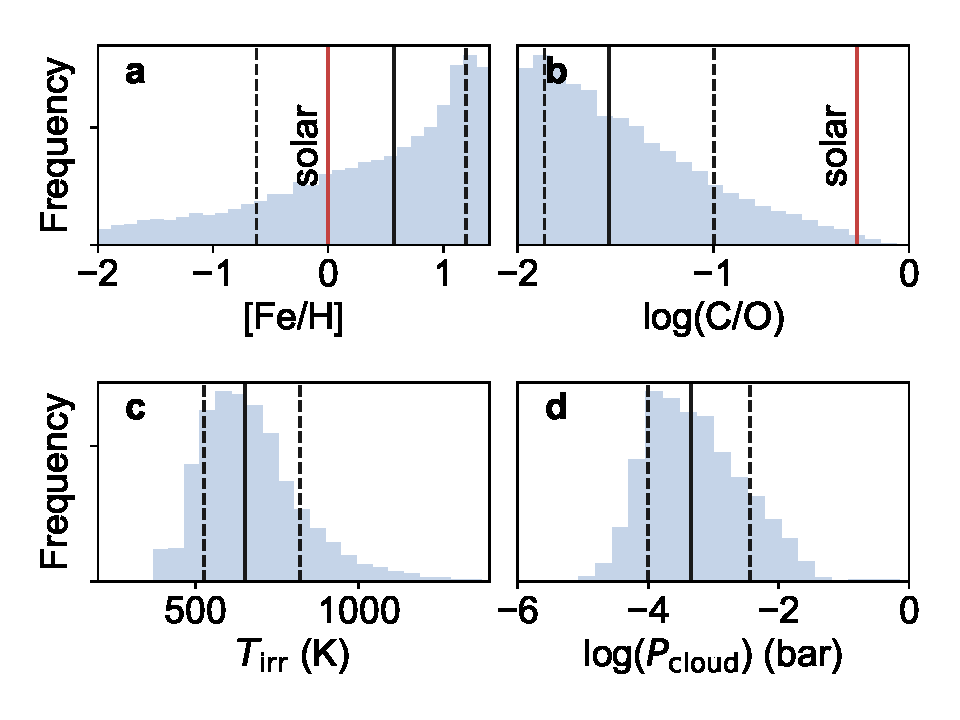
\includegraphics[width = 0.5\textwidth]{Figures/retrieval.pdf}
\caption{Retrieved distributions for (a) metallicity, (b) carbon-to-oxygen ratio, (c) irradiation temperature, and (d) cloud-top pressure in bars. Black vertical lines show the median and $\pm1\,\sigma$ confidence interval (solid and dashed, respectively). Solar metallicity and C/O values are indicated with red vertical lines.}  \label{fig:retrieval}
\end{figure}

\subsubsection{Methane Abundance}
We ran two additional retrievals to explore whether methane depletion is the underlying cause of the inferred low C/O.  Even though water is the dominant absorber in the WFC3 bandpass, there is enough methane opacity to change the shape of the spectral features at a detectable level for high precision data.  In one test, we assumed chemical equilibrium but excluded methane opacity. This set-up resulted in a much broader distribution of C/O values ($0.02 - 1.6$ at $1\,\sigma$). 

We also performed a ``free" retrieval that allowed the abundances of CH$_4$, H$_2$O and NH$_3$ to vary with no assumption of chemical equilibrium. The $3\,\sigma$ upper limit on methane abundance is $1.2\times10^{-3}$, ruling out the the predicted methane content for a composition with solar C/O and $3\,\times$ solar metallicity (the median metallicity from the chemical equilibrium retrieval).  Based on these tests, we conclude that the atmosphere of WASP-107b is depleted in methane relative to expectations for a solar abundance pattern. By contrast, the water abundance ($6\times10^{-6} - 2\times10^{-3}$) is consistent with predictions for solar composition.

\subsection{Condensate Properties}
In addition to the atmospheric retrieval, we also performed forward modeling of physically motivated, self-consistent clouds and hazes using the methods described in \cite{fortney08, morley15}.  We model clouds that form in cool atmospheres (Na$_2$S, KCl, ZnS; see \citealt{morley12}), for a range of metallicites from $1-50\times$ solar. We vary the cloud sedimentation efficiency from 3 to 0.1 (normal to highly lofted, small particulate clouds). None of the models produce sufficiently low amplitude spectral features to match the observed spectrum.  This result suggests that if clouds are muting WASP-107b's transmission spectrum, the mechanism for cloud particle formation and vertical lofting is very efficient and not captured by the modeling used here. Futher studies of cloud formation in very low gravity environments are required. 

We also model an \emph{ad hoc} photochemical ``soot" layer near the top of the atmosphere. We predict the abundance of hydrocarbon haze precursors from previously published photochemical models for GJ 436b \citep{line11, morley17}. With the most efficient haze production (100\% of precursors form haze) and particle sizes around $0.03-0.1$ microns, the amplitude of the model water feature matches that of the observations. 

These photochemical hazes are assumed to form from hydrocarbons generated by methane photolysis; however, we found in the previous section that methane is depleted.  Furthermore, even if the precursors were present, it is unclear whether the 100\% haze production efficiency is realistic.  However, organic hydrocarbons are not the only possible photolytic haze in cool H2-rich atmospheres, as sulfur chemistry may create additional haze material \citep{zahnle09, gao17}. Further modeling and laboratory work of the hazes that form in these conditions is needed for a satisfactory explanation of the data.  

\section{Discussion and Conclusions} \label{sec:discuss}
We analyzed the atmospheric composition of WASP-107b based on retrieval of its near-infrared transmission spectrum and interior structure models of the planet's mass and radius.  Key results from this analysis include:

\begin{itemize}
\item{\emph{The upper limit on atmospheric metallicity is $30\times$ solar.} This limit is at the edge of consistency with the Solar System metal enrichment trend, which predicts a metallicity of $30\times$ solar for WASP-107b \citep{kreidberg14b}.  Compared to results for other exoplanets of similar mass such as GJ 436b, which has a high metallicity ($>100\times$ solar) and HAT-P-26b, which is metal-poor compared to the Solar System trend, WASP-107b adds to the evidence that exoplanets exhibit a greater diversity of compositions than is present in the Solar System \citep{morley17, wakeford17}.}
\item{\emph{The methane abundance is depleted relative to expectations for a solar abundance pattern, whereas water is consistent with solar composition.} This may be due to an instrinsically low carbon-to-oxygen ratio, which could arise from accretion of water-rich planetesimals \citep{mordasini16, espinoza17}.  Another possibility is that the planet has a hot interior effective temperature ($\sim500$ K), and abundances are quenched at pressure levels where CO is stable \citep[as observed in some directly imaged planets;][]{skemer14, zahnle14}. Such a high internal temperature could be due to latent heat of formation if the planet is very young, and/or tidal heating \citep{fortney08, morley17}. Further observations of the transmission spectrum over a broader wavelength range will refine the C/O estimate and help differentiate between these two scenarios.} 
\item{\emph{Optically thick condensates are present at high altitudes} ($0.1 - 3$ mbar). The amplitude of the water absorption feature in the transmission spectrum is less than a third that expected for a clear atmosphere. Existing models of physically-motivated cloud and haze formation do not satisfactorily reproduce the data. All the cloud models  we consider produce condensation too deep in the atmosphere. Efficient hydrocarbon haze production at high altitudes can match the data, but these require the presence of methane to serve as a haze precursor.  Other precursors such as H$_2$S are a possibility and would be worth exploring in future analyses. Put in context with other systems, the muted water feature for WASP-107b agrees well with the trend in feature amplitude with temperature noted in \cite{crossfield17}, indicating that condensates may be common in the atmospheres of the coolest planets.}
\end{itemize}

These results are a first look at the atmosphere of WASP-107b. The planet is already being observed at other wavelengths, including the WFC3/G102 grism and Spitzer 3.6 and 4.5 $\mu$m channels in transit and eclipse (\emph{HST} Program GO 14916, PI J. Spake, \emph{Spitzer} Program 13052, PI M. Werner; \emph{Spitzer} Program 13167, PI L. Kreidberg).  In addition, WASP-107b is included in the \emph{JWST} Guaranteed Time Observations for the NIRISS, NIRCAM, and NIRSpec instruments\footnote{\url{https://jwst-docs.stsci.edu}}.  This spate of observing programs is sure to add to the already rich and complex picture of WASP-107b's atmosphere presented here. 


\acknowledgments
We thank Fei Dai, Jessica Spake, Ian Crossfield, Hannah Diamond-Lowe, and Jonathan Fortney for productive conversations. L.K. acknowledges support from the Harvard Society of Fellows and the Harvard Astronomy Department Institute for Theory and Computation. C.V.M. acknowledges support from NASA through the Sagan Fellowship Program.

\bibliographystyle{aasjournal}
\bibliography{ms.bib}

\end{document}

